\chapter{Flight Controller}

In this project several software approaches have been investigated for the flight controller. Three different concepts have been worked on to get the best results and answer questions regarding the characteristics of variable pitch quadrotors. An existing flight controller software has been modified to work with variable pitch. Another fully self-made flight controller has been created and tested, including an autonomous system, which works for each of the mentioned systems. \bigskip

Rapid development, multiple coding languages, different flight controllers and autonomous systems have increased the difficulty to keep a good coding standard. Version control have been facilitated using Github ensuring backup and traceability.

\section{Concepts}
%Bytt nummer på konsepter
In the initial description of the project it was suggested to use an open source flight controller called Pixhawk. The plan was to modify the Pixhawk to support variable pitch. Using the Pixhawk was discarded since it was considered to be difficult to work with. The solution was to build the flight controller from scratch using a microcontroller and keeping it as simple as possible.\bigskip

The team have access to a motion capture system called Qualisys located at KONGSBERG Innovation Center (KIC). The plan was to use this system to track the quadrotor and collect the necessary data to analyze both variable and fixed pitch quadcopters for comparison. Qualisys also gives the possibility of making an autonomous controller using the position data from the motion capture cameras as feedback. If autonomous flight is achieved, it will make testing more reliable without the errors of a human pilot.  \bigskip

\begin{figure}[H]
          \centering
            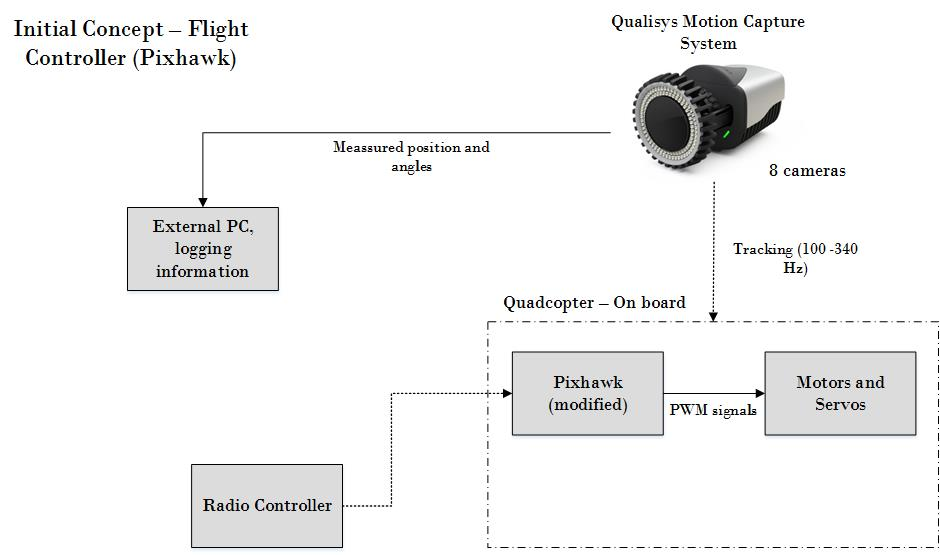
\includegraphics[scale = 0.45]{VAPIQ-PICTURES/Concept4.jpg}
                \caption{Initial Concept}
                \label{Con3}
            \label{dir}
\end{figure} 

During the early phases of the project, several concepts for the flight controller were considered. Below a description of the different concepts are given.

\clearpage

\subsection{Concept 1}

The first concept consists of using Qualisys as the only source of sensing and data collection. The computations for the quadcopter would be done on an external computer using Qualisys as the IMU. In this way, the need for on-board computations would be eliminated. The disadvantage of this concept, is that the team has limited access to KIC and would be dependent on doing all testing exclusively at KIC. 

In Fig. \ref{fig:OCO} the first concept is illustrated\\
\begin{figure}[H]
          \centering
            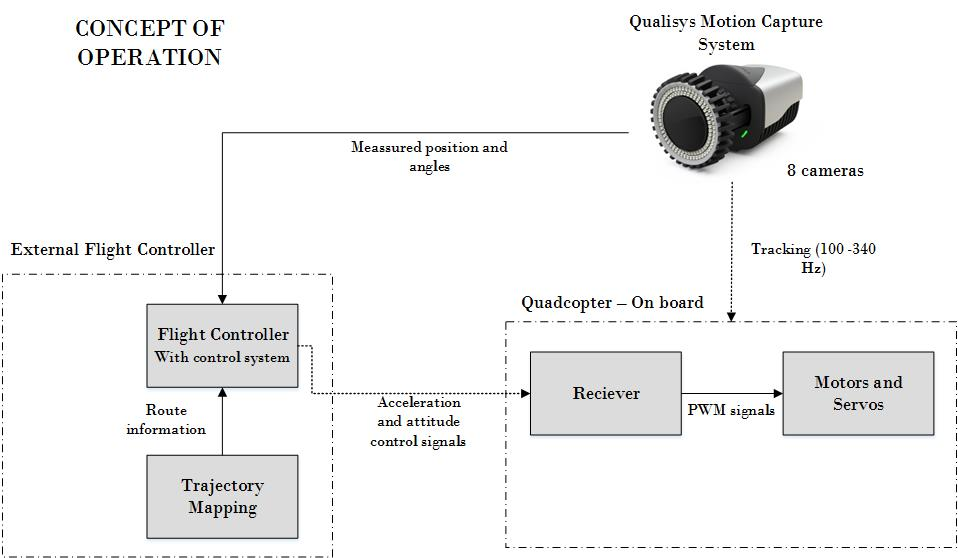
\includegraphics[scale = 0.6]{VAPIQ-PICTURES/ConceptOfOperation.jpg}
                \caption{Concept 1}
                \label{fig:OCO}
            \label{dir}
\end{figure}

Information is sent from Qualisys and received on an external computer where all calculations are performed. QTM provides six different values (x, y, z, $ \phi, $ $ \theta ,$ $ \psi $). These values describe the position and rotation of the quadrotor. By taking the information provided about its position and rotation, an algorithm determines the roll, pitch, yaw, and thrust change for each motor. The calculated values are translated into motor and servo signals which are sent back to the quadcopter for stabilization. \bigskip

The initial assumption was that this concept would simplify writing the flight controller software. The advantages of computing externally are increased computational power and less hardware and sensors on the quadcopter. \bigskip

However testing showed that the latency was too high. The Bluetooth signals alone used about 0.08s giving an update frequency of 12.5Hz, provided that the computation and Qualisys sampling happens instantly. With an update frequency of 12.5Hz or lower would limit the agility of the quadrotor and make stabilization very unlikely. The minimum acceptable time it can take for Qualisys to update, compute and send back the signals to the quadcopter cannot be more than 20ms. \bigskip

After analyzing this concept it became clear that it had to be discarded. Stabilization could be hard to achieve with frequencies below 50Hz.\\

\clearpage
%%%%%% Concept 2  %%%%%%%
\subsection{Concept 2}
The second concept proposed for the flight controller, see Fig. \ref{Con2}, consists of moving the control system to the quadrotor to do stabilization on-board. This would improve the inner control loop frequency. To accomplish this, an IMU and a processing unit must be placed on the quadcopter. The control loop would only need to sample data from the IMU, compute the desired changes on-board and update the motors and servos.

\begin{figure}[H]
          \centering
            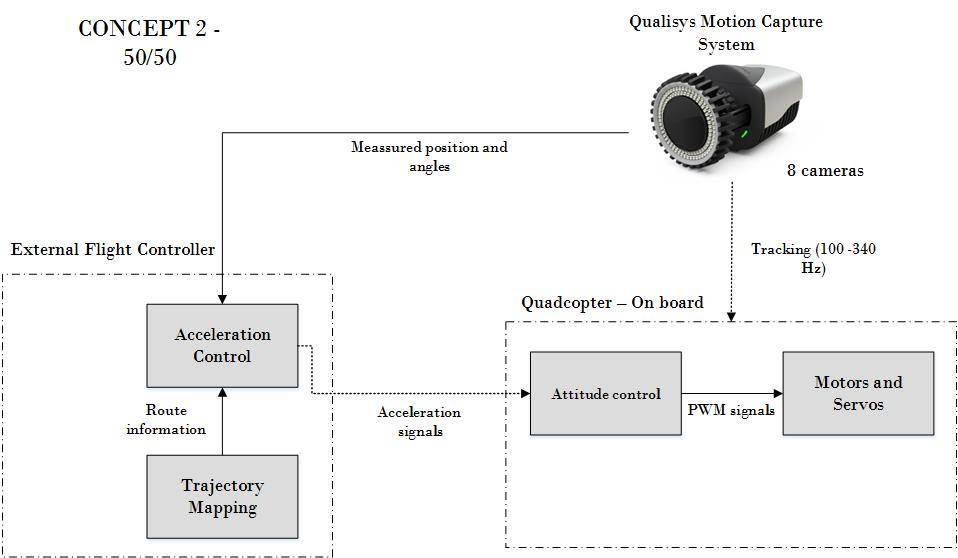
\includegraphics[scale = 0.67]{VAPIQ-PICTURES/Concept2.jpg}
                \caption{Concept 2}
                \label{Con2}
            \label{dir}
\end{figure} 
\\

In this concept the external computer would still control the position and trajectory of the quadcopter. This would keep the advantage of using Qualisys with trajectory planning for reliable and reproducible data. Additionally, it would give more computational power. This concept has, unlike the first concept, a fast control loop and it would also reduce the experienced drift over time because of the inputs given from Qualisys.\bigskip

%This is the concept that was chosen for the project.

%Bør være concept 4 for ryddighetens skyld.

\clearpage

\subsection{Concept 3}
The third concept, is to move all computations and position handling on-board the quadrotor, eliminating Qualisys as a sensing unit. This would yield a higher control loop frequency because the quadrotor does not have to receive information from Qualisys and the external computer. \bigskip

By using this concept, the trajectory is controlled by a pilot using a radio controller, instead of making the quadrotor autonomous. Qualisys would only be an observer, and the data produced is only dependent on the inputs of the pilot. \bigskip

Fig. \ref{Con3} shows Qualisys only as an observer. If Qualisys is to be used in this concept instead of the RC-pilot, it would be difficult to make trajectories because all movement would need to be pre-programmed as stick-inputs sent to the quadrotor. 

\begin{figure}[H]
          \centering
            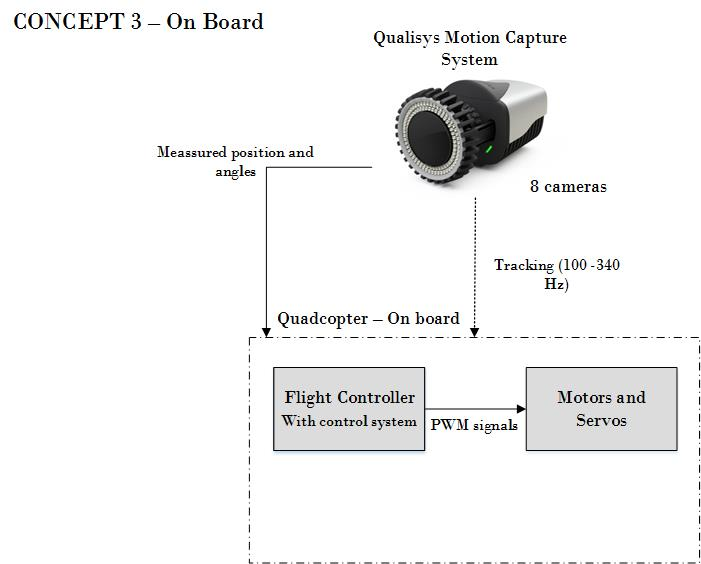
\includegraphics[scale = 0.67]{VAPIQ-PICTURES/Concept3.jpg}
                \caption{Concept 3}
                \label{Con3}
            \label{dir}
\end{figure} 

This is the concept that was chosen for this project. The main advantage with this concept is that Qualisys is not required to fly the quadcopter, so it can be tested at HSN without being solely dependant on access to KIC. \bigskip


\subsection{Concept Selection}

Concept three was chosen after an analysis. The autonomous system is not required in this concept. Using Qualisys only as an observer. Having everything on the quadcopter and only observing the system with Qualisys makes the autonomous system redundant. This seems to be the quickest way to get answers about the characteristics of variable pitch quadrotors. Results is more reliable if the human factor can be removed. If there is enough time, the autonomous system in concept two will be implemented and used for testing.

%The downside to this concept is that it requires more computation time and/or computation-power on-board the quadcopter. 


\section{Flight Controller with Radio Controller}

The final flight controller used in this project is based on Joop Brokkings \textbf{YMFC 3D - Your Multicopter Flight Controller}. \cite{joop}. This software has served as a foundation for the development of the variable pitch flight controller. The flight controller is as simple as possible and supports radio control. To ensure reliable data, the radio controller can be replaced by an autonomous control system using the motion capture system Qualisys at KIC. This will only be done if there is time. \bigskip

The flight controller software consists of four Arduino programs which are uploaded separately. A short description of each of them will follow.\bigskip

\textbf{Setup}\\
This is the first part, and is uploaded to the Arduino without the battery connected. When the sketch is uploaded a setup procedure is launched. This guides the user through a series of tasks to calibrate the quadcopter. The first step in setup is to calibrate the radio controller. The center values of the sticks are stored.
When the controller is calibrated, the setup will search for a IMU and start calibration of the gyroscope. The software stores the direction of the axis for roll, pitch and yaw. After everything is done, the stored values are written to the EEPROM to ensure that the other sketches can utilize the same configuration. \bigskip

\textbf{ESC Calibration}\\
This is a simple sketch to ensure that all of the ESCs are calibrated and that the motors starts at the same speed when activated. This part also contains a function that can help the user check if everything on the quadcopter is working properly. When the battery is connected, the user may spin one motor after the other to ensure correct rotational direction of each motor. The ESC calibration can also be used to balance the propellers.  \bigskip

\textbf{Servo Calibration}\\
To achieve stable flight, the pitch on all propellers must be mechanical zero-pitch. In servo calibration, each servo is manually set to zero-pitch and tuned by communication over the serial monitor. When the values corresponding to zero-pitch are found, they are stored and used as zero-reference in the main controller. \bigskip

\textbf{Flight Controller}\\
This is the main program and contains the actual flight controller software. The sketch reads the EEPROM to get the correct configurations of the quadcopter. Before the quadcopter is ready to fly, the IMU takes 2000 samples to calibrate the sensor and to calculate the average gyro offset. The quadcopter starts when the throttle stick is placed in the lower left corner and stops when the throttle stick is placed in the lower right corner. \bigskip

When the quadcopter is started, the motors will start spinning at minimum speed until more throttle is received from the radio controller. The receiver input signals operates on interrupts, this means that when a change is made to the controller all other programs running are paused to interpret the controller inputs.\bigskip

To take full advantage of variable pitch, the motors are running at a higher starting RPM than on a regular fixed pitch quadcopter. This is to ensure that as much kinetic energy as possible is stored in the rotating parts. In this way, pitch actuation will be able to unleash the kinetic energy resulting in high acceleration rates. The signals controlling the servos are mapped from the ESC-values, which have already been treated by the PID algorithm.\bigskip

Additionally, it has been implemented a debug function which helps detect errors in the controller if enabled.

\subsection{Libraries and Frequencies}
The flight controller software utilizes the Wire.h library in Arduino and communicates with the IMU on fast I2C running at 400kHz. The Servo.h library is used for controlling the servos, which is a standard Arduino library. The library has been changed to have higher refresh rates since the loop is running faster than 50Hz. The servos used are digital and capable of up to 333Hz. \bigskip

The main loop of the flight controller runs at a frequency of 250Hz, the gyroscope is sampled with a refresh rate of 1kHz but can be sampled with up to 8kHz. 
The increased sample rate of the gyro gives the possibility of filtering the gyro date without slowing down the main loop. Four samples of the gyro are taken and processed by a running average filter. The filtered values of the gyro are used in the PID calculation and are used to make corrections to the quadcopter. \\ 
\section{PID Tuning}
To achieve stable flight, the control system must be tuned properly. This is done by identifying the correct PID-values through a combination of methods, trial and error. In the flight controller, there are three PID-loops for each of the rotational directions; roll, pitch and yaw. \bigskip

The approach used to tune the PID-controller is given below:
\begin{itemize}
    \item \textbf{Yaw}
        \begin{itemize}
            \item  Eliminate uncontrolled yaw by increasing the proportional value by one, until yawing stops.
            \item  Increase the integral value by 0.01 to prevent yaw impact from small physical differences. 
            \item  For yaw, there is no need to change the derivative value because of the drag generated from the propellers.
        \end{itemize}
    \item \textbf{Roll and Picth} are given the same value unless the quadrotor has a CG outside of physical center.
        \begin{itemize}
            \item The derivative value is increased by one until the quadrotor shows high frequency oscillations, then lowered down until the quadcopter runs smooth again. The value is then reduced by 25\%. 
            \item The proportional value is increased by 0.2 until the quadrotor starts to overcompensate, then divide the value by 2.
            \item The integral value is changed by 0.01 until the quadrotor starts to oscillate, then divide by 2.
            \item Increasing the proportional value until fast oscillation occur, and subtract a few points until the quadcopter is fully stable. 
        \end{itemize}
\end{itemize}

By following these steps, the quadrotor should be stable and able to fly. To get the variable pitch properly tuned, the method above was applied and additional advise was taken from a professional RC pilot. The final PID settings for the variable pitch quadrotor for pitch and roll are (11.5, 0.03, 10) and the values for yaw are (18, 0.04, 0) \cite{PID-tune}.
\clearpage



\clearpage   %% Starts new page



\newpage
%%%%%%%%%%%%%%%%%%%%%%%%   Autonomous System %%%%%%%%%%%%%%%%%%%%%%%%%%%%%%%%%%%%%%%%%%
\chapter{Autonomous System}

In this project, it has been a goal to implement autonomy. If the autonomy is implemented it will give reproducible test flights and ensure consistency without a human error.  There has been developed several applications that might work, but has not yet been tested due to lack of time. \bigskip

The working of the planned autonomous system is given below.

\section{On-Board - second concept}
%concept to, på quadcopteret?

For the autonomous system to work, there has to be an on-board chip on the quadcopter. This chip will compute the inner control loop responsible for stabilization. In the on-board code multiple libraries are used. Servo.h for servo control of pitch and SoftwareSerial.h for bluetooth communication. On-board the quadcopter, trajectories are received from the external computer via bluetooth. The external computer is also connected to the motion capture system Qualisys to monitor and track the quadcopter.


\subsection{Calibration - Arming and Sensor Readings}

When the quadcopter is started the sensors have to be calibrated. 1000 samples of the gyro data is taken to calculate and calibrate for the offset. Under calibration it is imperative that the quadcopter is at rest, or else any disturbances will offset the calibration. Under startup the quadrotor must be placed in zero degrees, else the calibration will set zero-level at an incline and the quadcopter will not work properly.\bigskip

Calibrating the 9250 MPU sensor improved the accuracy of the readings by a factor of 250, it has reduced angular velocity start error from $\pm$ 10 deg/(deg/s) to $\pm$ 0.04. When calibration is finished, a LED is lit and the quadrotor waits for a bluetooth signal matching its start protocol. 
When the start signal is received the quadrotor will arm the motors by sending PWM signals to each motor (1000$\mu$s).\bigskip

When activation is completed, the quadrotor enters the control loop. Here, the IMU gets read and the readings goes through a lowpass filter and a weighted moving average filter. Filtering is done to remove most of the vibration noise created by the propellers. The filtered data then gets saved to an array and are fed back to the PID-algorithm every 20ms. 

%This process is repeated until it has taken a given amount of samples (currently set to five samples, this will however change soon). \\

%If no such signal is sent, then it reads the gyro and accelerometer data. 

%This data gets c

\section{External Autonomous Control}

The external computer acts as an off-board flight controller. It deals with tracking the position and the information provided from Qualisys to control the trajectory of the quadcopter. The external control system, is written in python and can give the needed pitch and roll angles to make the quadrotor follow the specified path. The off-board control system logs information with a logging function in python. This function gives debug, warning and critical messages. \bigskip  

A challenge with the Qualisys software is that it provides the first measured data. The information needed to stabilize the quadrotor is however, the most recent. To solve this, multi-threading was used. This works by keeping a separate function constantly updating this information. In this way current position and rotation is always available. \bigskip

%Position, rotation and trajectory of the quadrotor is measured by Qualisys. 
%The main goal with the off-board controller is to provide the quadrotor with the information required to keep a specified path. 

\subsection{Establishing Connection}
The off-board code first tries to establish connection with Qualisys. If no contact is achieved it will not start. To establish connection and to start the quadcopter a two-way handshake is performed.

\subsection{Communication With Off-Board}
Communication with the quadrotor can be done by either bluetooth or RF signals. Only one of the devices will be used at once. Information is sent by using a string which contains the angles, rotation and thrust. The string gets interpreted when it reaches the Arduino and gets cast into an integer.

\subsection{Safety Mechanism}
%Multiple mechanisms have been created to ensure safety of the quadrotor, facility and the people involved. \\
%The code checks if a bluetooth signal is sent to turn it off. If no off signal has been sent, then PWM (1000$\mu$s) signals are sent to each motor. If such a signal is received it breaks out of the inner-loop and waits for a new starting signal. \\

When flying autonomously in Qualisys, a safety mechanism is present. The quadrotor has a given area that it can fly in, specified in the code. If the quadrotor moves out of this scope in either the x, y or z axis, it will automatically shutdown. The software constantly checks if the quadrotor is within the specified boundary. The control system also constantly checks if it has lost connection, if connection is lost the system will shut-down.